\section{\textit{Synthesizing Parameterized Motions}}

% ============================================================================
\subsection{Referência completa do artigo}

\begin{itemize}
  \item \textbf{Autores:} Michiel van de Panne, Ryan Kim, Eugene Fiume
  \item \textbf{Local:} University of Toronto
  \item \textbf{\textit{Journal}:} Eurographics
Workshop on Animation and Simulation [Qualis : não encontrei]
  \item \textbf{Data:} Sept. 17-18, 1994
  \item \textbf{Referência:} \citeonline{bib:1994:synthesizing}
\end{itemize}


% ============================================================================
\subsection{Resumo}

%Máquinas de estado finito são utilizadas para alternar entre parâmetros de controle, para permitir movimentações cíclicas mais complexas, e decisões de novas poses podem ser tomadas baseadas em dados obtidos por sensores.
\subsubsection{Abstract}

In striving to construct higher level control representations for simulated characters or creatures, one must seek flexible control representations to build upon. We present a method for the synthesis of parametrized, physics-based motions. The method can be applied to both periodic and aperiodic motions. The basis of the method is a low-level control representation in which linear combinations of controllers generally produce predictable in-between motions.

% ..........................................................
\subsubsection{Propósito do artigo}

O artigo propõe um método de gerar movimentos realisticos de forma reusável e parametrizada, isto é, evitando que o problema de controle tenha de ser resolvido novamente para cada novo caso específico.

Existem diversas técnicas de animação para gerar tais movimentos. O autor optou pelo uso de controladores, onde há uma informação de como o movimento deve ser realizado, mas respeitando restrições como a física, causando um aumento de realidade na ação. 

Um controlador pode ser tornado mais versátil adicionando a capacidade de parametrização de seus atributos, e podem receber informação do ambiente, permitindo reações a estímulos externos durante a movimentação.

% ..........................................................
\subsubsection{Técnicas utilizadas} 
\begin{itemize}
  \item Controladores PD
  \item Máquinas de estado finito
  \item Algoritmos Genéticos
  \item Otimização em duas fases
  \item Arrefecimento simulado
  \item Método do gradiente
\end{itemize}  

% ..........................................................
\subsubsection{Contribuição em relação a artigos anteriores} %mais ou menos 10 linhas
 \begin{itemize}
   \item Um estudo anterior havia sido feito para casos em que a movimentação era exclusivamente cíclica. O artigo expande essa noção para aplicar a qualquer topologia de grafo de pose.
   \item O poder computacional necessário para sintetizar uma solução foi drasticamente reduzido em relação a mais de uma solução anterior.
 \end{itemize}  

% ============================================================================
\subsection{Metodologia}
% Descreva um pouco mais detalhadamente a metodologia e os resultados do artigo. 
% Inclua as figuras que achar mais relevantes.

\subsubsection{Grafos de controle de pose}

Máquinas de estado finito são utilizadas para alternar entre parâmetros de controle, para permitir movimentações cíclicas mais complexas. Decisões de novas poses também podem ser tomadas baseadas em dados obtidos por sensores.

Uma pose é definida por um conjunto de graus de liberdade do modelo.

%A figura \ref{fig:1994:synthesizing:fig1} ilustra um grafo de pose e o tempo de transição entre cada estado.

\begin{figure}[ht]
  \centering
  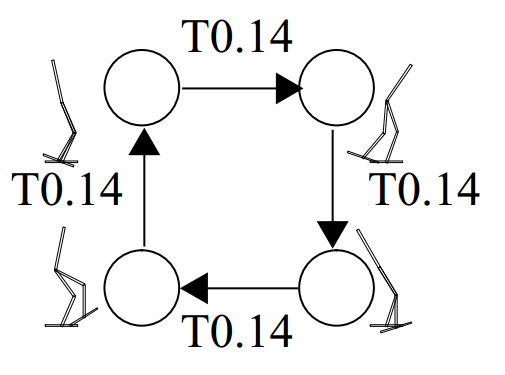
\includegraphics[height=100px]{artigos/1994_Synthesizing_Parameterized_Motions_egw94/fig1.png}
  \caption{Grafo de pose com tempo de transição entre os estados.}
  \label{fig:1994:synthesizing:fig1}
\end{figure}

\begin{figure}[ht]
  \centering
  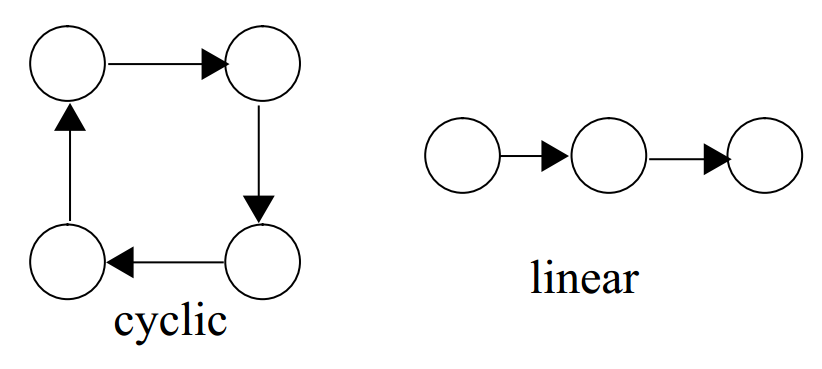
\includegraphics[height=100px]{artigos/1994_Synthesizing_Parameterized_Motions_egw94/fig2.png}
  \caption{Duas possíveis topologias para o grafo de pose.}
  \label{fig:1994:synthesizing:fig2}
\end{figure}

Grafos de pose são grafos orientados que representam as transições entre as diferentes configurações desejadas do modelo articulado.

Os parametros dos controladores podem ser definidos manualmente ou sintetizados. No artigo, o autor cita o uso da técnica de otimização em duas fases para gerar os parâmetros. Então é gerado um grafo de controle da pose, onde cada estado representa uma posição no qual o controlador deverá tentar atingir. As posições são representadas por um conjunto de graus de liberdade dos atuadores, que contém informação dos valores máximos e mínimos para cada um, como visto na figura \ref{fig:1994:synthesizing:fig12}.

\begin{figure}[ht]
  \centering
  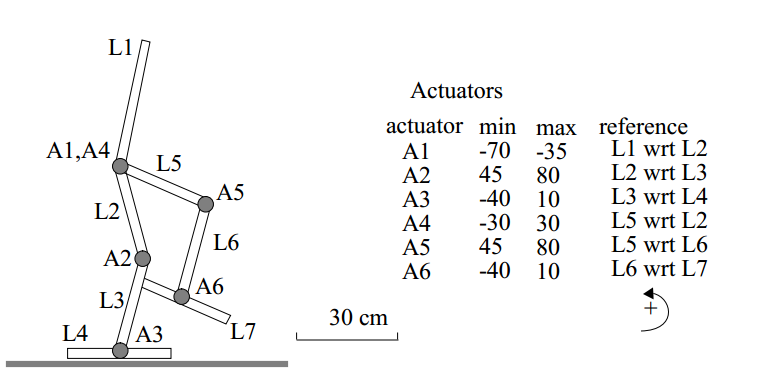
\includegraphics[height=150px]{artigos/1994_Synthesizing_Parameterized_Motions_egw94/fig12.png}
  \caption{Modelo simples com duas pernas representando o "estado zero" e todos os graus de liberdade para atingir a pose vista.}
  \label{fig:1994:synthesizing:fig12}
\end{figure}

Os experimentos foram realizados utilizando um modelo 2D, porém o autor demonstra otimismo para expandir a técnica para um modelo 3D. Para atingir maior realismo da simulação, o modelo deve ser mais discretizado e contar com mais tipos de atuadores para ter uma melhor representação da musculatura do individuo.

Para criar uma animação, um animador precisa primeiramente criar uma figura articulada, especificar a topologia do grafo de controle de pose e decidir qual métrica será usada para avaliar o desempenho da animação. Essa métrica normalmente é uma combinação de valores como velocidade, distância percorrida e energia consumida no processo.

Para movimentos periódicos, um grafo cíclico é necessário. Dado um período desejado T e um numero n de transições, o tempo de transição é calculado fazendo $ \frac{T}{n} $. Para movimentos aperiódicos, um grafo linear é definido a priori.

Essas informações são utilizadas para reduzir drasticamente o espaço de busca, e consequentemente o tempo, do processo de síntese. O processo de síntese produz uma pose para cada estado do gráfico que gere uma animação desejada.

A técnica de busca utilizada, em duas fases, consiste em gerar controladores, testá-los, e a partir dos resultados, modificá-los e testá-los novamente até que um resultado desejado seja atingido. Os controladores gerados são avaliados através da métrica definida inicialmente. 

\begin{figure}[ht]
  \centering
  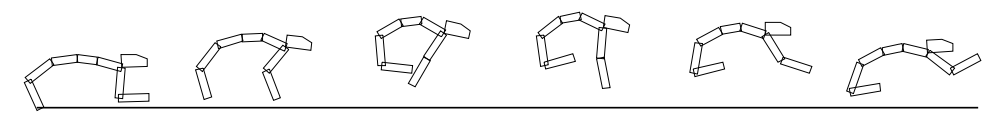
\includegraphics[width=300px]{artigos/1994_Synthesizing_Parameterized_Motions_egw94/fig3.png}
  \caption{Modelo de cheetah exemplificando o resultado de um movimento cíclico.}
  \label{fig:1994:synthesizing:fig3}
\end{figure}

Para um caso de teste, foram gerados na primeira fase 100 controladores, dos quais apenas 10 foram selecionados para prosseguir. Para a segunda fase, parâmetros dos controladores foram perturbados utilizando um delta fixo de 5\% o valor da amplitude do grau de liberdade, aleatoriamente. Então é decidido se a mudança será mantida ou não, baseado novamente na métrica. Para conseguir tais resultados, arrefecimento simulado ou método do gradiente podem ser utilizados.
O resultado pode ser observado na figura \ref{fig:1994:synthesizing:fig3}.

\begin{figure}[ht]
  \centering
  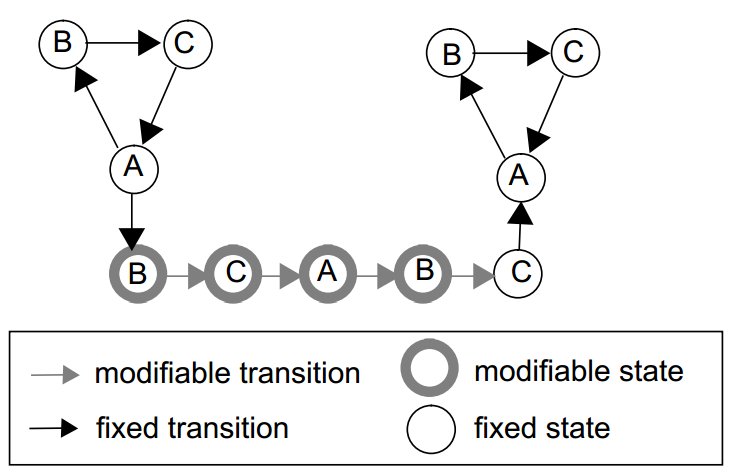
\includegraphics[height=100px]{artigos/1994_Synthesizing_Parameterized_Motions_egw94/fig4.png}
  \caption{Grafo de controle de pose representando o salto do Luxo, mascote da Pixar.}
  \label{fig:1994:synthesizing:fig4}
\end{figure}

Muitos movimentos aperiodicos interessantes podem ser derivados a partir de movimentos periódicos. Na figura \ref{fig:1994:synthesizing:fig4}, vemos que existe uma porção cíclica, representando um movimento periódico. Dado uma condição, é possível sair do ciclo através da transição do meio, e retornar em seguida. Dessa forma, Luxo faz um movimento de saltos, e pode interromper o ciclo para fazer um pulo longo, e retornar ao seu movimento anterior.

%parametrização de movimento

Parametrização de movimento é uma forma de abstrair todos os possíveis tipos de movimentação. É um passo necessário para construção de mecânicas de controle mais complexas abstraindo determinadas noções de movimento. O animador já tem o poder de influenciar o resultado da animação modificando o modelo utilizado e a métrica da otimização. 

A relação entre os parâmetros do grafo de controle de posição e a animação resultante é bastante complexa. Dada a dificuldade de descrever essa relação de forma analítica, podemos observar o impacto que determinadas mudanças têm no resultado final da simulação. O que observamos é que pequenas mudanças nos parâmetros causam pequenas mudanças no movimento final. Como resultado dessa propriedade, podemos interpolar duas posições desejadas interpolando seus parâmetros de controle.

\begin{figure}[ht]
  \centering
  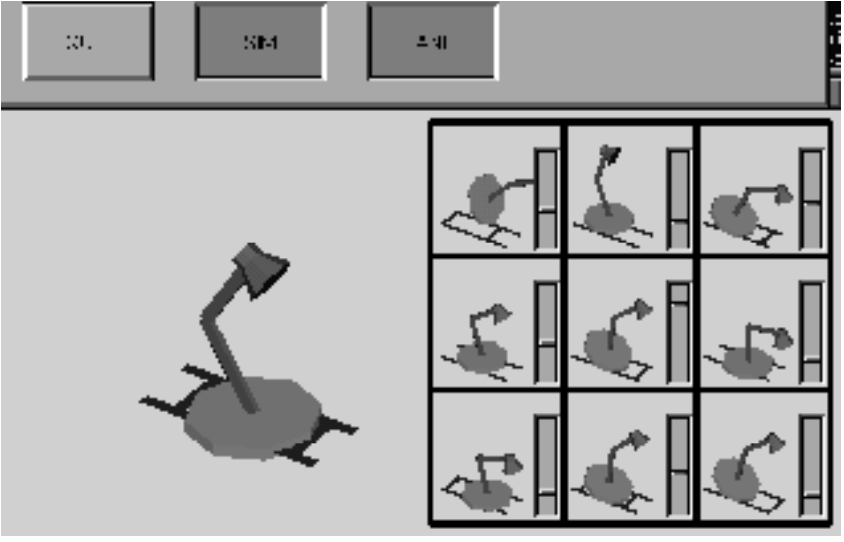
\includegraphics[height=150px]{artigos/1994_Synthesizing_Parameterized_Motions_egw94/fig10.png}
  \caption{É possivel ver no espaço da esquerda o movimento original de Luxo. Na direita, uma paleta de sugestões de possíveis modificações que podem ser feitas na animação.}
  \label{fig:1994:synthesizing:fig10}
\end{figure}

Uma forma de gerar variações do movimento é sortear um parâmetro por vez, e modificá-lo até que um critério de semelhança entre as posições não seja mais atendida.
O artigo cita o uso da velocidade como critério de semelhança, onde uma diferença de até +-30\% é classificada como semelhante.

Assim que as variações de movimento são geradas, o resultado pode ser utilizado como uma "paleta" de poses, como ilustrado na figura \ref{fig:1994:synthesizing:fig10} para o animador, interativamente, definir o comportamento desejado da animação. 

É importante notar que o resultado da interpolação dos parâmetros é diferente do caso em que se interpola valores cinemáticos. No caso da interpolação dos parâmetros, as leis da física serão mantidas no resultado final.

%\begin{figure}[ht]
%  \centering
%  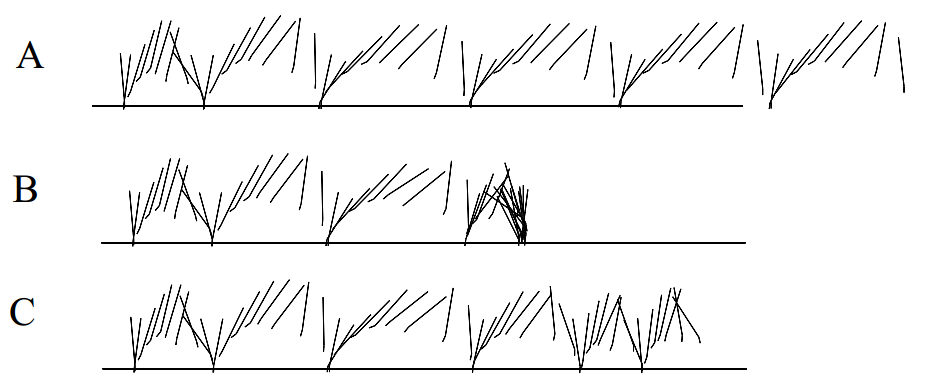
\includegraphics[height=100px]{artigos/1994_Synthesizing_Parameterized_Motions_egw94/fig6.png}
%  \caption{xxx}
%  \label{fig:1994:synthesizing:fig6}
%\end{figure}
%
%\begin{figure}[ht]
%  \centering
%  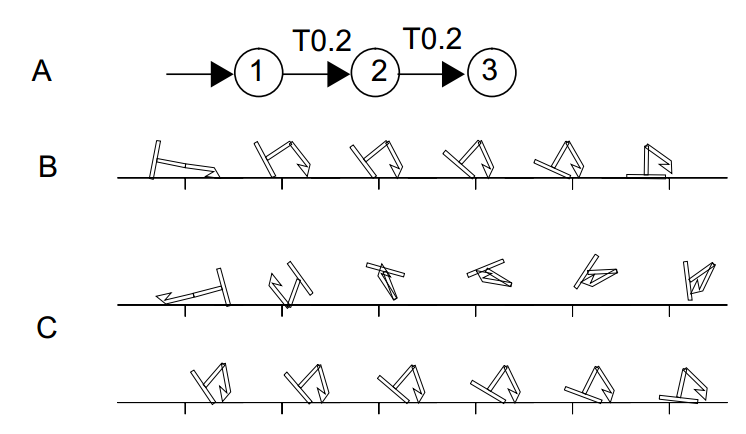
\includegraphics[height=100px]{artigos/1994_Synthesizing_Parameterized_Motions_egw94/fig7.png}
%  \caption{xxx}
%  \label{fig:1994:synthesizing:fig7}
%\end{figure}
%
%\begin{figure}[ht]
%  \centering
%  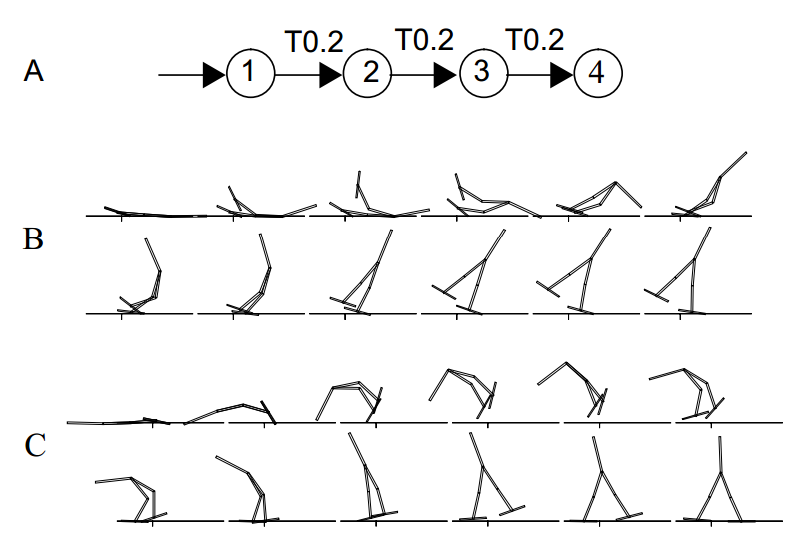
\includegraphics[height=100px]{artigos/1994_Synthesizing_Parameterized_Motions_egw94/fig8.png}
%  \caption{xxx}
%  \label{fig:1994:synthesizing:fig8}
%\end{figure}
%
%\begin{figure}[ht]
%  \centering
%  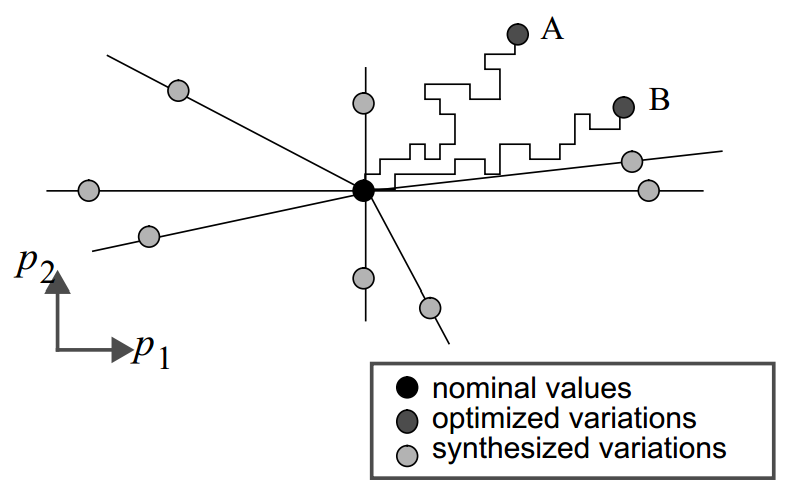
\includegraphics[height=100px]{artigos/1994_Synthesizing_Parameterized_Motions_egw94/fig9.png}
%  \caption{xxx}
%  \label{fig:1994:synthesizing:fig9}
%\end{figure}
%
%\begin{figure}[ht]
%  \centering
%  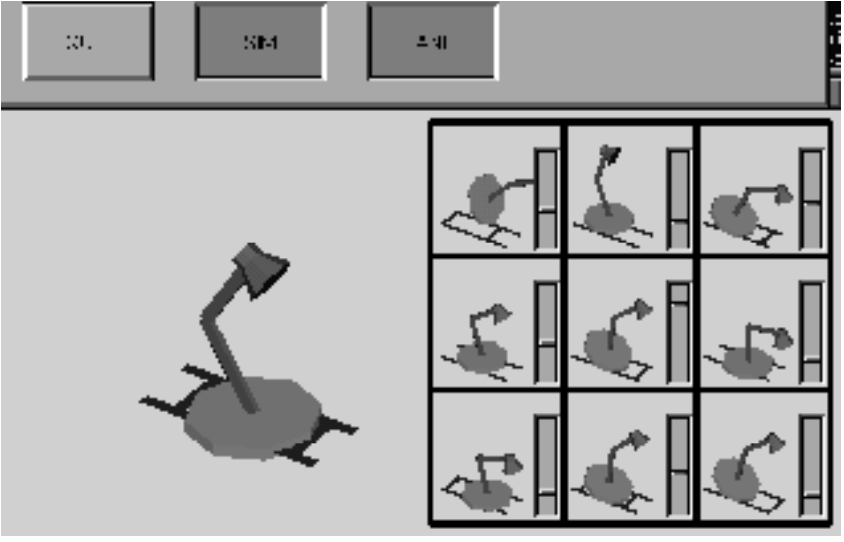
\includegraphics[height=100px]{artigos/1994_Synthesizing_Parameterized_Motions_egw94/fig10.png}
%  \caption{xxx}
%  \label{fig:1994:synthesizing:fig10}
%\end{figure}
%
%\begin{figure}[ht]
%  \centering
%  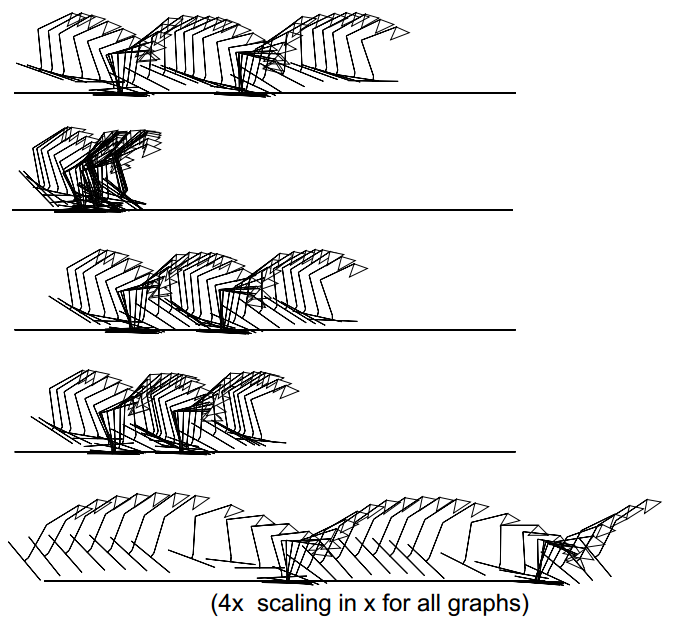
\includegraphics[height=100px]{artigos/1994_Synthesizing_Parameterized_Motions_egw94/fig11.png}
%  \caption{xxx}
%  \label{fig:1994:synthesizing:fig11}
%\end{figure}

% ..........................................................
\subsubsection{Resultados}
O uso de grafo de controle de pose demonstrou ser uma representação flexivel para criação de movimentos periódicos e aperiódicos. Quando usado com transições de estado baseados em tempo, pode gerar movimentos complexos que são graciosos e realistas.
Uma nova forma de utilizar otimização para sintese de movimento foi apresentada, melhorando aspectos como a criação de movimentos fisicamente realistas mais complexos, ciclicos ou aciclicos, de forma eficiente. Isso facilita o processo de projetar o controlador em alto nivel e os movimentos baseados em física.

% ============================================================================
\subsection{Pontos fortes} %no máximo três
\begin{itemize}
  \item Nova forma de utilizar otimização para síntese de movimentos.
  \item Grafo de controle de pose mais complexos, para movimentos cíclicos e aciclicos.
  \item Parametrização da solução que tornou possível um controle de mais alto nível sobre a simulação.
\end{itemize}  

% ============================================================================
\subsection{Limitações} %no máximo três
\begin{itemize}
  \item Movimentos que não são dinamicamente estáveis sem o uso de feedback não podem ser controlados em um ciclo fechado. Tais movimentos complexos necessitam de feedback contínuo do estado.
  \item A sintese do grafo de controle da pose continua um processo caro computacionalmente.
  \item 
\end{itemize} 


% ============================================================================
\subsection{Avaliação}
%\textbf{(a) Avanço considerável (\textit{Breakthrough}).}
 \textbf{(b) Contribuição significativa.}
% \textbf{(c) Contribuição modesta.}
% \textbf{(d) Contribuição fraca.}
% \textbf{(e) Sem contribuição.}
É possivel agora gerar movimentos fisicamente realistas com um algoritmo relativamente genérico. Dadas as restrições da técnica, é possível com algumas parametrizações gerar um grafo de controle de pose que resulte na animação desejada, sem a necessidade de manipular o grafo explicitamente.

Alguns artigos anteriores já haviam tentado algo parecido, porém com mais limitações na técnica e com desempenho inferior.

% ============================================================================
\subsection{Problema em aberto}
 \begin{itemize}
   \item Adicionar equilibrio resolveria o problema dos movimentos complexos?
   \item Otimizar o processo de sintese do grafo de controle de pose.
   \item Como conseguir movimentos mais autonomos e complexos com a sintese
   \item Extender a técnica para movimentos e modelos mais complexos e utilizando 3 dimensões ao invés de 2.
   \item Explorar a melhor forma de integrar informação sensorial aos grafos de controle de pose.
 \end{itemize}  

% ============================================================================
\subsection{Aspecto obscuro}
 \begin{itemize}
   \item É preciso ver como a técnica se comporta em animações de objetos mais complexos, ou seja, objetos com mais graus de liberdade.
 \end{itemize}  